%UNSW Thesis Template

\newif\ifdigital
\digitaltrue  %\toggle between digitaltrue and digitalfalse for paper vs didital copy

\ifdigital
  \documentclass[oneside,11pt,a4paper] {report} 

  \usepackage{fancyhdr,ifthen}

  % Setup for headers and footers (fancyhdr)
  \fancyhf{}
  \fancyheadoffset{0cm}
  \renewcommand{\headrulewidth}{0pt}
  \lhead{\ifthenelse{\isodd{\value{page}}}{\rightmark}{\leftmark}}
  \rhead{\thepage}
  \pagestyle{fancy}
\else
  \documentclass[twoside,11pt,a4paper,openright] {report} 
  \pagestyle{headings}
\fi

\usepackage{calc}
\newlength{\reqOddMargin}
\newlength{\reqEvenMargin}
\newlength{\reqTopMargin}
\newlength{\reqBottomMargin}

% UNSW specifications
% 40mm left-hand margin is require
% I am using 30mm
% Requires \paperwidth - (\reqOddMargin + \reqEvenMargin) = 158.75mm
% \paperwidth = 210mm

\ifdigital
  %%%%%%%%%%%%%%%%
  %  Digital specifications
  %%%%%%%%%%%%%%%%
  \setlength{\reqOddMargin}{25.625mm} % Should be >40mm
  \setlength{\reqEvenMargin}{25.625mm} %Should be >20mm
  \setlength{\reqTopMargin}{35mm} %Should be >30mm
  \setlength{\reqBottomMargin}{33.4mm} %Should be >20mm
\else
  %%%%%%%%%%%%%%%%
  %  Print specifications
  %%%%%%%%%%%%%%%%
  \setlength{\reqOddMargin}{32.25mm} % Should be >40mm
  \setlength{\reqEvenMargin}{19mm} %Should be >20mm
  \setlength{\reqTopMargin}{35mm} %Should be >30mm
  \setlength{\reqBottomMargin}{33.4mm} %Should be >20mm
\fi

% Functions to set the thesis to UNSW specifications
\setlength{\hoffset}{\reqOddMargin - 1in}
\setlength{\voffset}{\reqTopMargin - (1in + \topmargin + \headheight + \headsep)}
\setlength{\textheight}{\paperheight - \reqTopMargin - \reqBottomMargin}
\setlength{\textwidth}{\paperwidth - \reqOddMargin - \reqEvenMargin}
\setlength{\oddsidemargin}{0.0mm}
\setlength{\evensidemargin}{\reqEvenMargin - \reqOddMargin}

\usepackage{amsmath}
\usepackage{amssymb}
\usepackage{amsthm}
\usepackage{delarray}
\usepackage{amsfonts}
\usepackage{cite}
\usepackage{bm}
\usepackage{pdfpages}
\usepackage{pstricks}
\usepackage{pst-plot}
\usepackage{pst-eps}
\usepackage{pst-grad}
\usepackage[chapter]{algorithm}
\usepackage{algcompatible}
\usepackage{multirow}
\usepackage{eurosym}
\usepackage{graphicx}
% \usepackage{subfigure}
\usepackage{caption}
\usepackage{subcaption}
\usepackage{multirow}
\usepackage{lscape}
\usepackage{rotating}
\usepackage{afterpage}
\usepackage{acronym}
\usepackage{intcalc}


%Adjusting float parameters
\renewcommand{\textfraction}{0.05}
\renewcommand{\topfraction}{0.95}
\renewcommand{\bottomfraction}{0.95}
\renewcommand{\floatpagefraction}{0.5}

%Adding hyperlinks
\ifdigital
  \usepackage[ps2pdf,
  bookmarks=true,
  bookmarksnumbered=false, % true means bookmarks in
  % left window are numbered
  bookmarksopen=false, % true means only level 1
  % are displayed.
  colorlinks=true,
  linkcolor=red,
  citecolor=red,
  linktoc=none]{hyperref}
  \definecolor{webgreen}{rgb}{0, 0.5, 0} % less intense green
  \definecolor{webblue}{rgb}{0, 0, 0.5} % less intense blue
  \definecolor{webred}{rgb}{0.5, 0, 0} % less intense red
\fi

\linespread{1.5}


\allowdisplaybreaks[1]
% \usepackage[toctitles]{titlesec} 

% This package is used to compile all figures and tables at the end of the document.  - Good for checking the float captions and details.
% \usepackage{endfloat}
% \renewcommand{\efloatseparator}{\mbox{}}

\setcounter{secnumdepth}{2} %change this for more subsection options


%Commands for the table of acronyms
%Ensuring that CHAPTER x. TITLE only appears on chapter numbers greater than 0
\renewcommand{\chaptermark}[1]{%
\ifnum\value{chapter}>0
\markboth{\thechapter{}. \MakeUppercase{#1}}{}%
\else
\markboth{\MakeUppercase{#1}}{}%
\fi} 

%Changing the font of the acronym to be normal instead of bold
\renewcommand\acsfont{\normalfont}


%%%%%%%%%%%%%%%%%%%%%%%%%%%%%%%%%%%%%%%%%%%%%%%
%       Parameters for paragraph lengths
%%%%%%%%%%%%%%%%%%%%%%%%%%%%%%%%%%%%%%%%%%%%%%%
\newcommand{\tempparskip}{0pt}
\setlength{\parskip}{0pt plus 0.5pt minus 1.0pt}

%Spaces below floats
\newcommand{\squeezeup}{\vspace{-7mm}}
\newcommand{\semisqueeze}{\vspace{-3mm}}
\newcommand{\pressdown}{\vspace{3mm}}

%change this t have path refs rather than using /folder/folder/fig.eps
% \graphicspath{{pathname}}

%the bellow comments are for using 'trackchange' like comments in latex
\newcommand{\todo}[1]{\par\vspace{2mm} \noindent
\marginpar{to do}
\framebox{\begin{minipage}[c]{0.85\textwidth}
\tt #1 \end{minipage}}\vspace{2mm}\par}

\newcommand{\comment}[1]{\par\vspace{2mm} \noindent
\marginpar[\hfill Comment]{Comment}
\framebox{\begin{minipage}[c]{0.85\textwidth}
\tt #1 \end{minipage}}\vspace{2mm}\par}

\newcommand{\alignName}[2]{\parbox{\textwidth}{\parbox[l]{0.0001\textwidth}{\noindent(#1)}\parbox[l]{0.967\textwidth}{ #2 }}}

\newcommand{\mustreview}{\marginpar{\emph{must \\ review}}}
\newcommand{\tocheck}{\marginpar[\hfill\emph{check}]{\emph{check}}}
\newcommand{\reviewedpara}{\marginpar{\emph{paragraph \\ reviewed}}}
\newcommand{\reviewed}{\marginpar{\emph{reviewed}}}
\newcommand{\etal}[1]{\emph{et al.}\cite{#1}}

\providecommand{\tightlist}{%
  \setlength{\itemsep}{0pt}\setlength{\parskip}{0pt}}

%End of preamble
%______________________________________________________________________%

\date{}

\begin{document}

% titlepage! ===========================================================
\begin{titlepage}
  \pagestyle{empty}
  \begin{center}
    \includegraphics[width=4cm]{$logo$}
  \end{center}
  \vskip 2cm

  \begin{minipage}{0.85\textwidth}
    \vskip 0.9cm
      \begin{center}
        {\rmfamily\LARGE\bf\expandafter{$title$}}
      \end{center}
  \end{minipage}

  \vskip 1.5cm

  {\sc\rmfamily\Large\bf $author$}\\

  {\rmfamily\large Supervisors: $for(supervisors)$$supervisors$\\*$endfor$}\\

  \vskip 2.0cm
  {\rmfamily\large $division$ \\ School of $school$ \\ $institution$ \\ $location$}

  \vfill
  \begin{minipage}{0.8\textwidth}
    \begin{center}
      {\rmfamily A thesis submitted for the degree of \bf{$degree$} at
      $institution$.}
      \vfill
      {$date$}
    \end{center}
  \end{minipage}
\end{titlepage}

\newpage

% unsw coversheet and statements
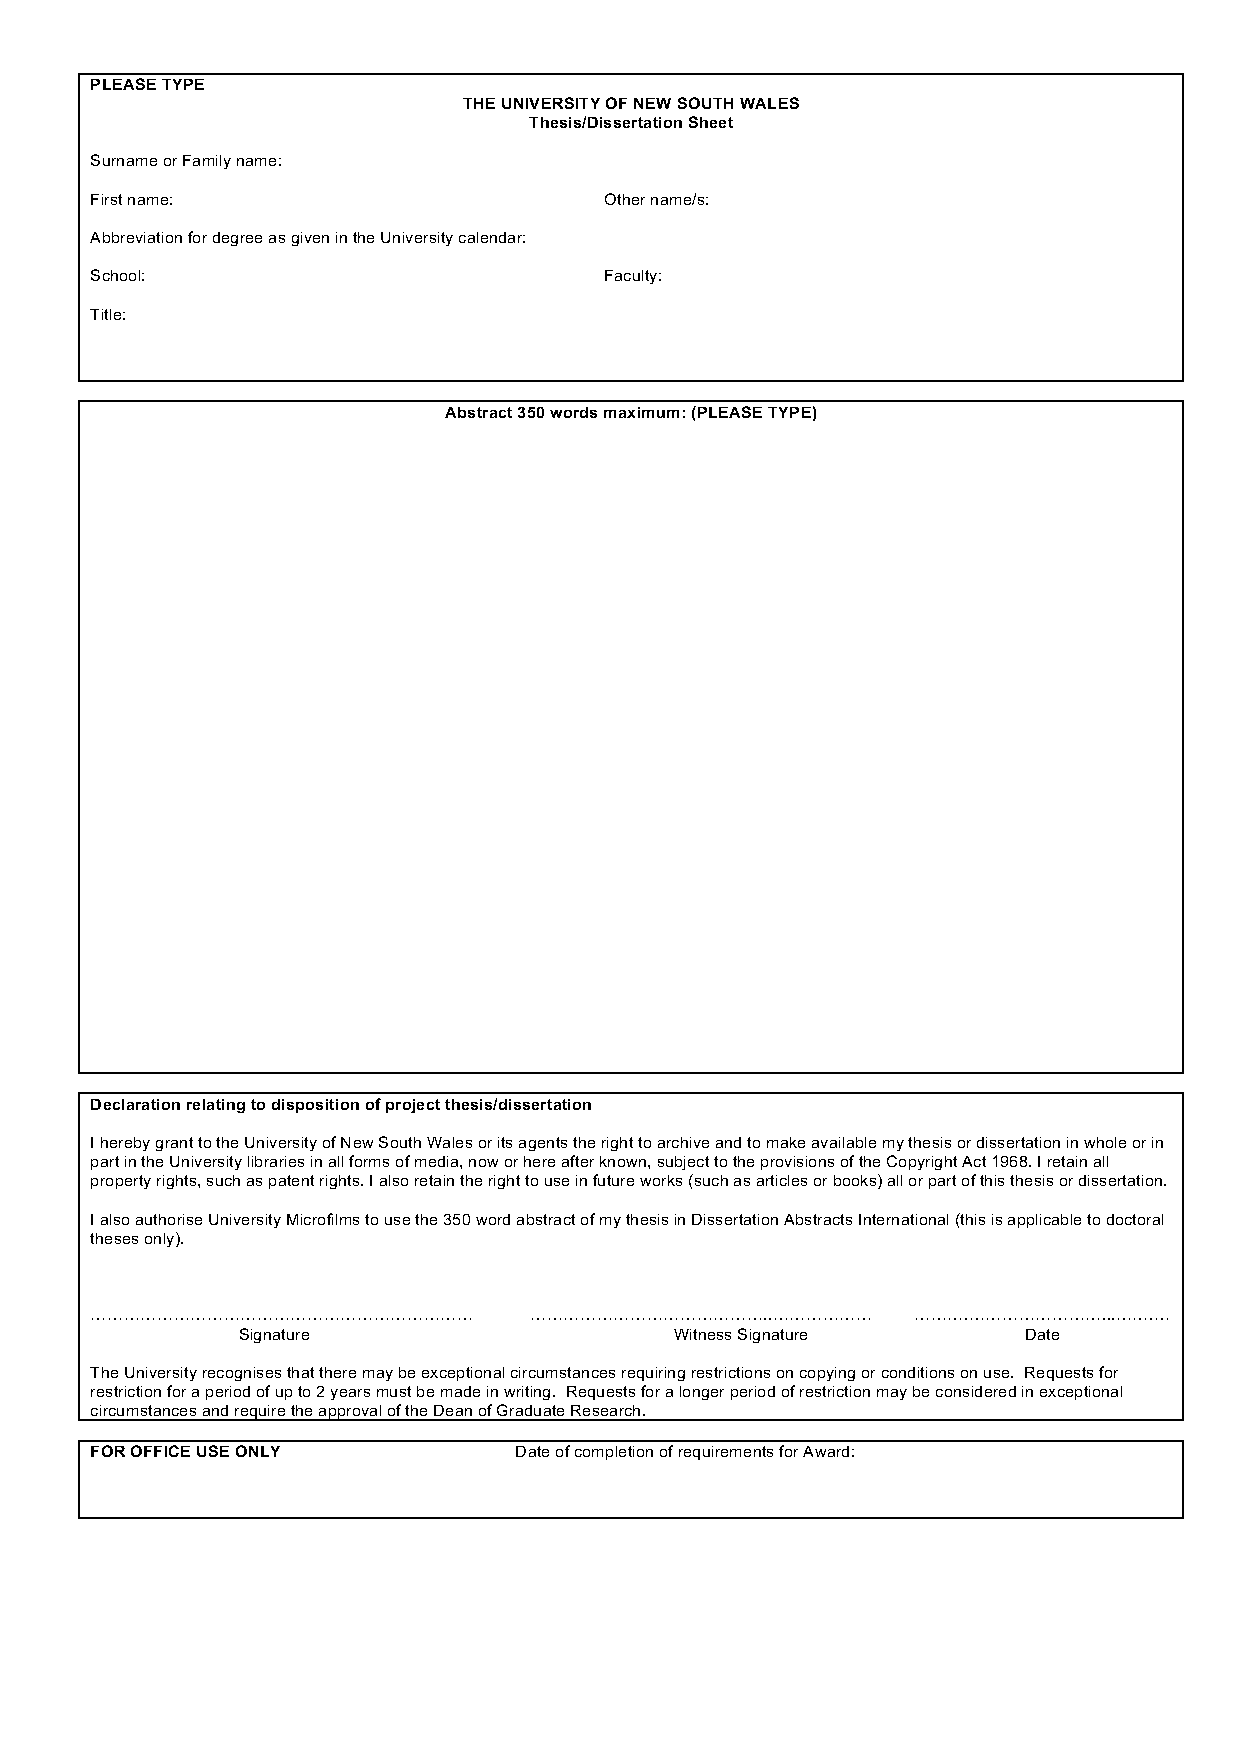
\includepdf[pages=-, offset=0 0]{forms/coversheet.pdf}
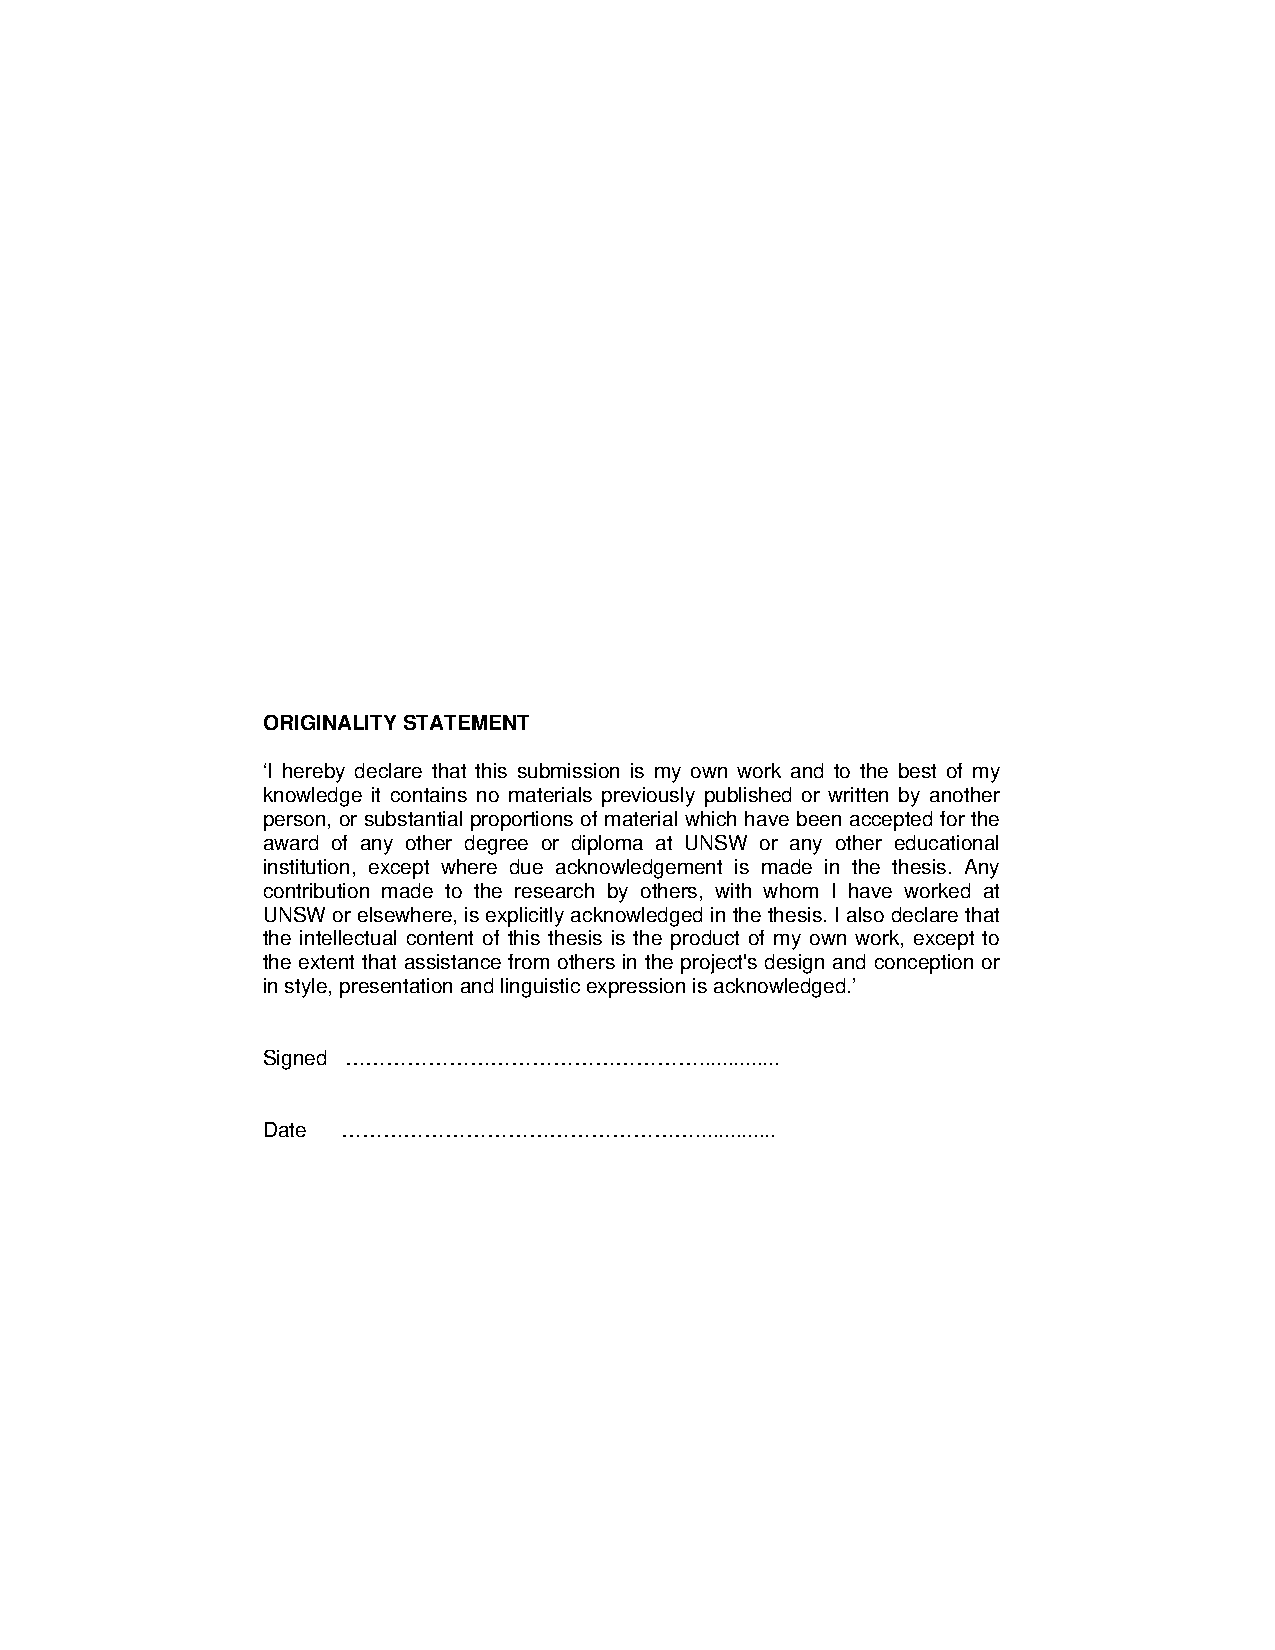
\includepdf[pages=-, offset=0 0]{forms/originality.pdf}
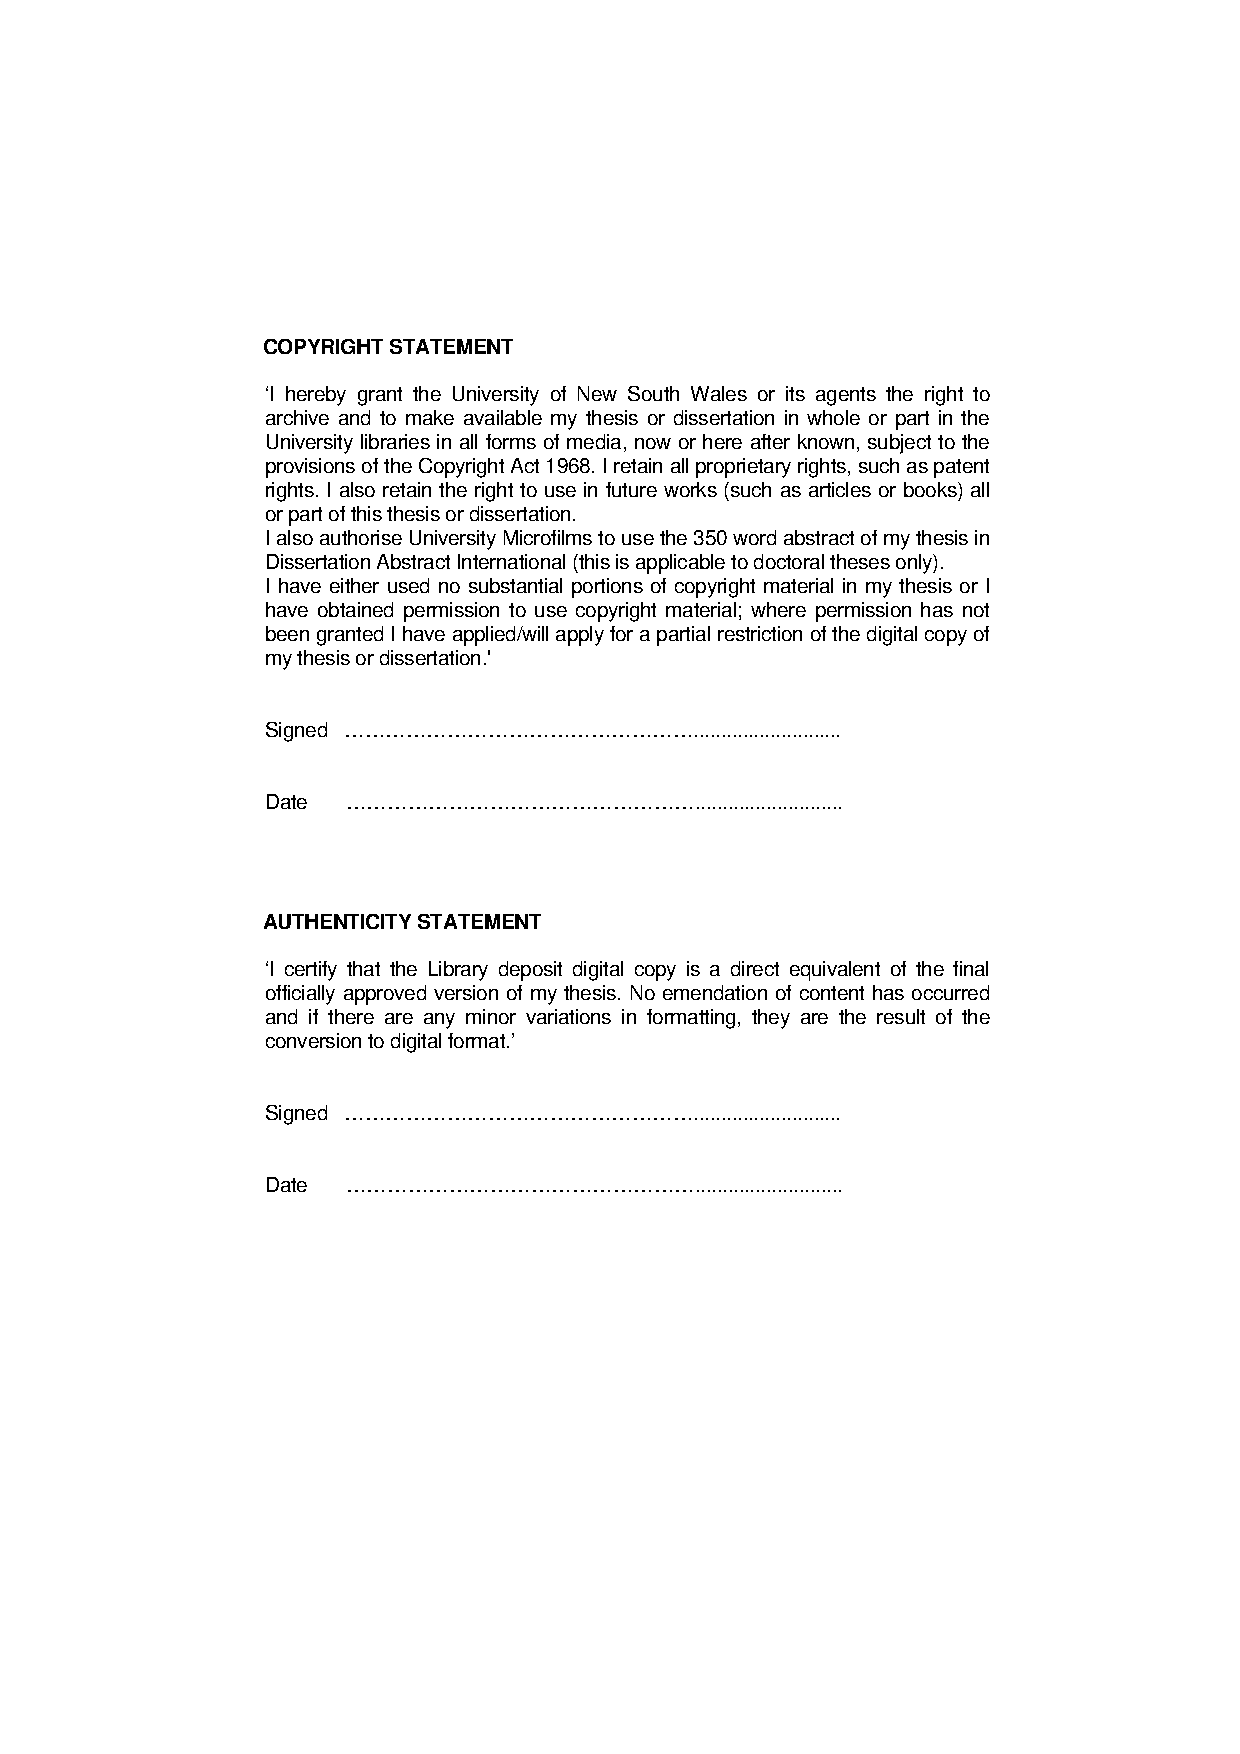
\includepdf[pages=-, offset=0 0]{forms/copyright-authenticity.pdf}

\cleardoublepage

% abstract =====================================================================
$if(abstract)$
  \ifdigital
    \pdfbookmark{Abstract}{Chap:Abs} 
  \fi
  \begin{abstract}
    \pagestyle{empty}
    $abstract$
  \end{abstract}

  \newpage
  \thispagestyle{empty}
  \cleardoublepage
$endif$

% acknowledgements =============================================================
$if(acknowledgements)$
  \renewcommand{\abstractname}{Acknowledgements}
  \ifdigital
    \pdfbookmark{Acknowledgements}{Chap:Ack} 
  \fi
  \begin{abstract}
    \pagestyle{empty}
  $acknowledgements$
  \end{abstract}

  \newpage
  \thispagestyle{empty}
  \cleardoublepage
$endif$

% dedication ===================================================================
$if(dedication)$
  \renewcommand{\abstractname}{dedication}
  \ifdigital
    \pdfbookmark{Dedication}{Chap:Ded} 
  \fi
  \begin{abstract}
    \pagestyle{empty}
  $dedication$
  \end{abstract}

  \newpage
  \thispagestyle{empty}
  \cleardoublepage
$endif$

% ------------------

\pagenumbering{roman}
\setcounter{page}{1} 

\tableofcontents

\cleardoublepage
\ifdigital
  \phantomsection 
\fi
\addcontentsline{toc}{chapter}{\listfigurename}
\listoffigures

\cleardoublepage
\ifdigital
  \phantomsection 
\fi
\addcontentsline{toc}{chapter}{\listtablename}
\listoftables

\newpage

\pagenumbering{arabic}
\setcounter{page}{1}

$body$

% bibliography commented out; knitr should handle this w/ 99-references.Rmd

% \ifdigital
%   \cleardoublepage
%   \phantomsection 
%   \pdfbookmark{Bibliography}{Chap:Bib}   
% \fi

% %change bibliography to the path of your file filename.bib
% \bibliography{filename}
% \bibliographystyle{abbrv}


\end{document}


